\documentclass[10pt,a4paper]{article}

\bibliographystyle{ieeetr}

\usepackage[margin=1in]{geometry}
\usepackage{graphicx}
\usepackage{subfig}
\usepackage{amsmath}
\usepackage{url}
\usepackage{pgfgantt}
\usepackage{lscape}
\usepackage{pdfpages}
% \usepackage{diagbox}

\graphicspath{{./figs/}}

\newcommand{\code}[1]{\texttt{#1}}

\title{A modular kernel for the Raspberry Pi: Progress Report}

\begin{document}

\maketitle

\begin{center}
    Thomas Archbold \\
    1602581 \\
    University of Warwick \\
\end{center}

\section{Introduction}
% problem that project addresses, motivations (importance of undertaking)
% make sure objectives are clear and clarify why it is a significant undertaking
% and of suitable level for third year project in computer science

\section{Background}
% all research I have put into it until this point - good understanding of
% background and how it fits into landscape (does not exist in isolation, before
% or after conception)
% indication of how background information was gained - a few citations that
% have been key sources for project

\section{Current progress}
The project is currently at a point at which the operating system is able to
successfully boot in the emulated environment provided by QEMU. Since it has
been capable of doing this since \code{boot.s} was written, early on in Term 1,
it is important to note the specific stages of initialisation performed by the
kernel at this point, as well as discuss the environment setup that has enabled
this point in development to be reached.

\subsection{Development environmet}
The project is being developed on a machine running Linux kernel version 4.16
onwards. Since the target environment, the Raspberry Pi 2 Model B, is different
to that on which it is being developed, a cross-compiler is required to compile
code that will run on the target machine, as opposed to the host. In particular,
available for download on the ARM developer website \cite{GNUtoolchain} is the
GNU Embedded Toolchain, which provides tools to target ARM Cortex family of
processors, including the GNU Compiler Collection (GCC). Conveniently this suite
of tools is available from Arch Linux's package manager, pacman, and this is the
version of the cross-compiler used in the makefile.

\subsection{Makefile}

\subsection{linker.ld}
\subsection{boot.s}
\subsection{Atags}
\subsection{Initialising memory}
\subsection{Printing to HDMI}
\subsection{Booting on real hardware}

% overview of work so far, including
%   technical content - what work have I done, meaningful summary of significant
%   aspects
%   progress - review progress against timetable. If unexpected delays, how have
%   they been dealt with?

\section{Next steps}
% outline plans for next term and any alterations to original ideas
% updated timetable with as much detail as possible

\section{Reflection}
% reflection and appraisal - assessment on how thing shave gone so far. Any
% lessons learned to make future progress smoother?

\section{Ethical consent}
% state that I have considered it, but not needed

\section{Project management}
% How have I managed the project so far - may use formal methodology (e.g.
% management of code versions), and can refer to less formal ways of keeping on
% track, e.g. regular meetings with supervisor

\bibliography{bibliography}

\appendix

% include project specification as part of appendices
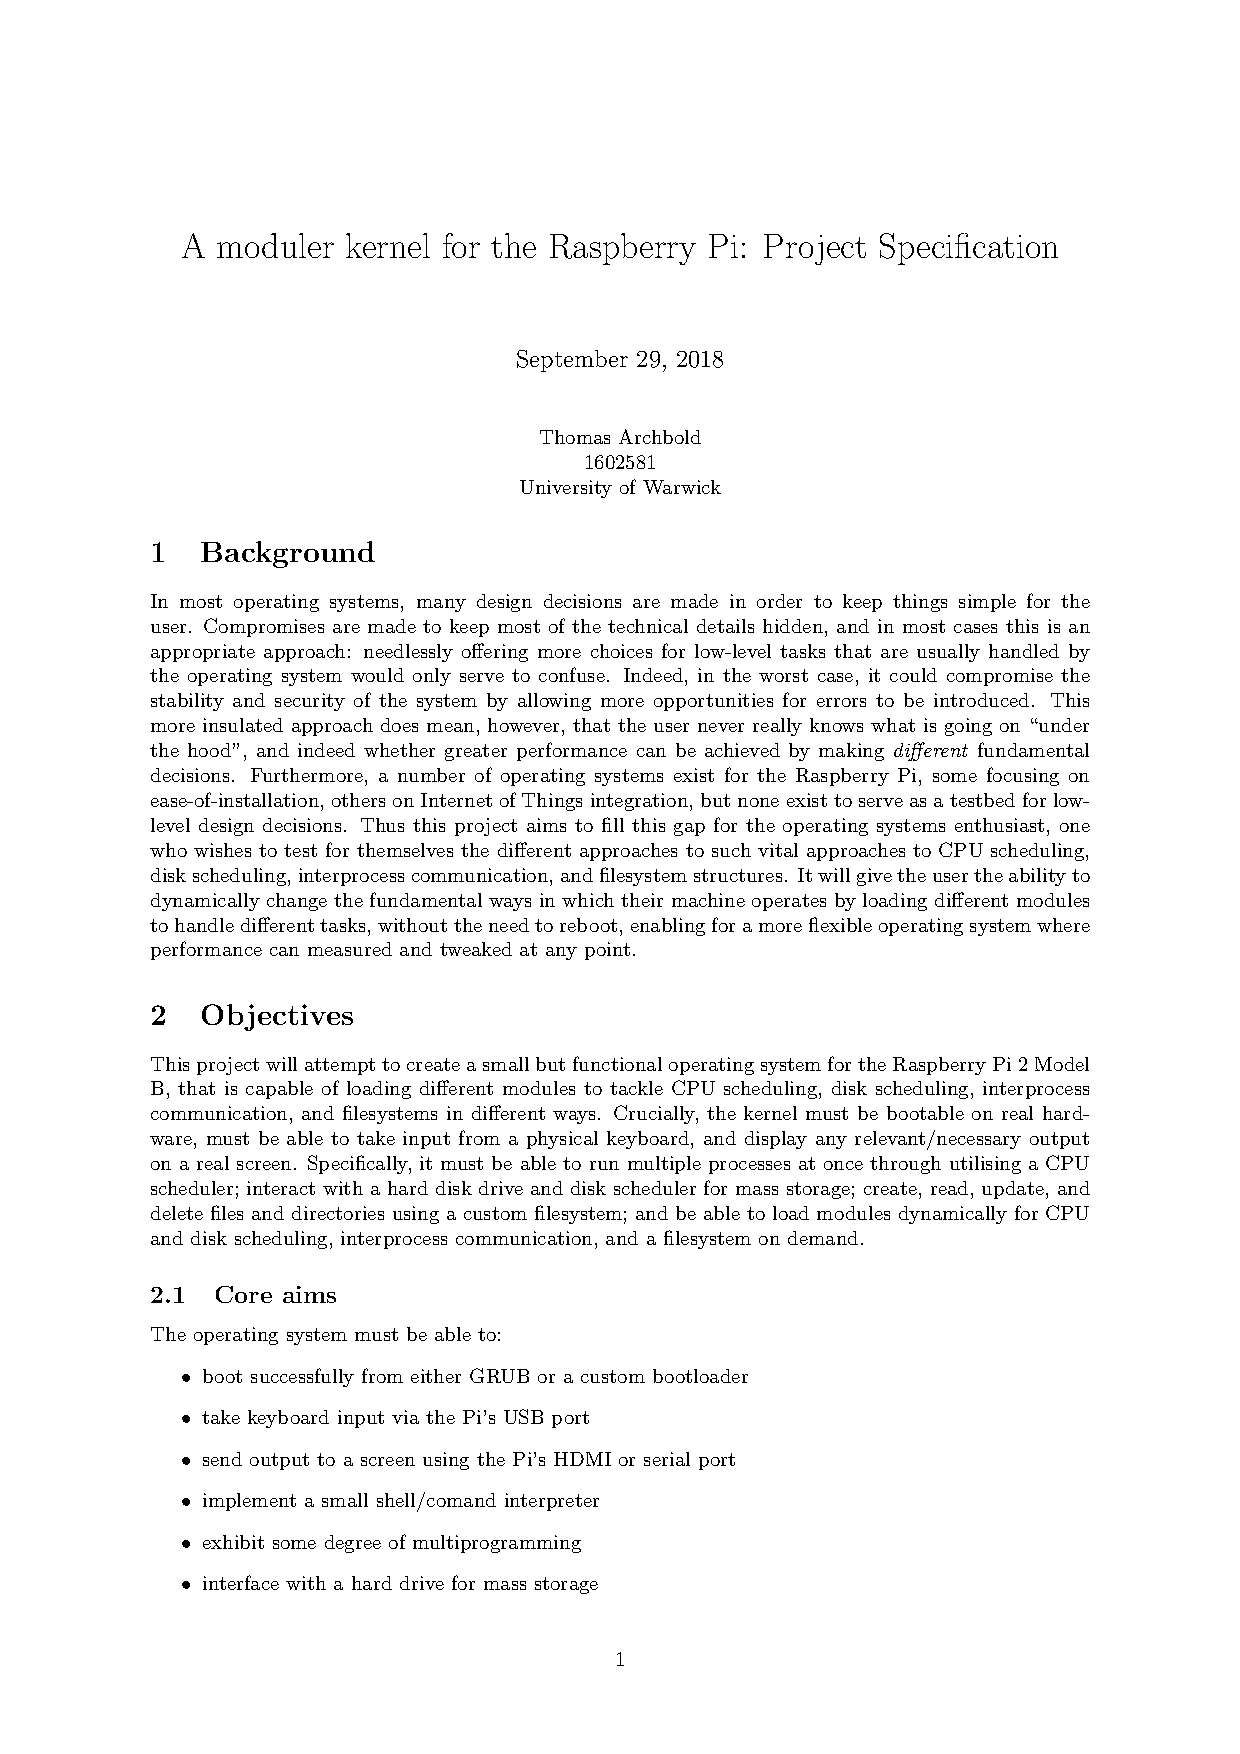
\includepdf[pages=-]{../specification/specification.pdf}

\end{document}
